% !TEX root=./adl.tex

% -----------------------------------------------------------------------
\begin{frame}{Context Parallelism --- Motivation}

  \emphdef{Context Parallelism} (CP) splits the \textbf{input sequence} across GPUs to handle long contexts~\cite{liu2023ring}.

  \vspace{0.3em}
  \begin{center}
  \begin{tikzpicture}
    \def\cs{0.5} % cell size

    % ===== Top row: full sequence on 1 GPU =====
    \foreach \i in {0,...,3}   { \fill[green!25]  ({-4+\i*\cs},0) rectangle ++(\cs,\cs); }
    \foreach \i in {4,...,7}   { \fill[violet!25] ({-4+\i*\cs},0) rectangle ++(\cs,\cs); }
    \foreach \i in {8,...,11}  { \fill[orange!25] ({-4+\i*\cs},0) rectangle ++(\cs,\cs); }
    \foreach \i in {12,...,15} { \fill[cyan!25]   ({-4+\i*\cs},0) rectangle ++(\cs,\cs); }
    \foreach \i in {0,...,15}  { \draw ({-4+\i*\cs},0) rectangle ++(\cs,\cs); }
    % Sparse token labels
    \node[font=\tiny] at ({-4+0.25},0.25) {$x_1$};
    \node[font=\tiny] at ({-4+0.75},0.25) {$x_2$};
    \node[font=\tiny,gray] at (0,0.25) {$\cdots$};
    \node[font=\tiny] at ({4-0.25},0.25) {$x_s$};
    % Brace below full sequence
    \draw[decorate,decoration={brace,amplitude=3pt,mirror},thick,gray]
      (-4,-0.08) -- (4,-0.08) node[midway,below=4pt,font=\tiny,gray] (stok) {};
    \node[font=\tiny,gray,left=0.1cm of stok] {$s$ tokens};

    % ===== Arrow =====
    \draw[->,very thick,>=stealth,green!50!black] (0,-0.42) --
      node[right,font=\tiny,green!50!black] {~CP: split along $s$} (0,-0.82);

    % ===== Bottom row: split across 4 GPUs =====
    \def\by{-1.3}
    % GPU 0: x from -4.45 to -2.45
    \foreach \i in {0,...,3} {
      \fill[green!25] ({-4.45+\i*\cs},\by) rectangle ++(\cs,\cs);
      \draw ({-4.45+\i*\cs},\by) rectangle ++(\cs,\cs);
    }
    \node[font=\tiny\bfseries] at (-3.45,{\by+0.25}) {GPU 0};
    % GPU 1: x from -2.15 to -0.15
    \foreach \i in {0,...,3} {
      \fill[violet!25] ({-2.15+\i*\cs},\by) rectangle ++(\cs,\cs);
      \draw ({-2.15+\i*\cs},\by) rectangle ++(\cs,\cs);
    }
    \node[font=\tiny\bfseries] at (-1.15,{\by+0.25}) {GPU 1};
    % GPU 2: x from 0.15 to 2.15
    \foreach \i in {0,...,3} {
      \fill[orange!25] ({0.15+\i*\cs},\by) rectangle ++(\cs,\cs);
      \draw ({0.15+\i*\cs},\by) rectangle ++(\cs,\cs);
    }
    \node[font=\tiny\bfseries] at (1.15,{\by+0.25}) {GPU 2};
    % GPU 3: x from 2.45 to 4.45
    \foreach \i in {0,...,3} {
      \fill[cyan!25] ({2.45+\i*\cs},\by) rectangle ++(\cs,\cs);
      \draw ({2.45+\i*\cs},\by) rectangle ++(\cs,\cs);
    }
    \node[font=\tiny\bfseries] at (3.45,{\by+0.25}) {GPU 3};
    % s/N_CP brace under GPU 0
    \draw[decorate,decoration={brace,amplitude=3pt,mirror},thick,green!50!black]
      (-4.45,{\by-0.08}) -- (-2.45,{\by-0.08})
      node[midway,below=4pt,font=\tiny,green!50!black] {$s / N_{\text{CP}}$};
  \end{tikzpicture}
  \end{center}

  \vspace{0.1em}
  \begin{columns}
    \begin{column}{0.48\textwidth}
      \textbf{Problem: Activation memory}
      \begin{itemize}
        \item TP shards along $h$, but $s$ remains full
        \item Sequence Parallelism (SP) only shards \emph{element-wise} ops --- attention requires every token to attend to every other, so SP cannot help there
      \end{itemize}
    \end{column}
    \begin{column}{0.48\textwidth}
      \textbf{Key insight:}
      \begin{itemize}
        \item Flash Attention computes attention \emph{block by block} via online softmax
        \item The blocks don't need to be on the same GPU!
        \item Each GPU holds $s / N_{\text{CP}}$ tokens and streams $K,V$ from other GPUs
      \end{itemize}

      \vspace{0.3em}
      \textbf{What is sharded?}
      \begin{itemize}
        \item \textbf{Activations} (along sequence dim) $\checkmark$
        \item Weights replicated (or via TP/ZeRO)
      \end{itemize}
    \end{column}
  \end{columns}
\end{frame}

% -----------------------------------------------------------------------
\begin{frame}{Ring Attention --- Core Idea}

  \emphdef{Ring Attention}: arrange CP group in a \textbf{ring}, pipeline $K,V$ transfers with local FlashAttn.

  \vspace{0.2em}
  \begin{center}
  \scalebox{0.95}{%
  \begin{tikzpicture}[
    gpu/.style={draw, rounded corners, minimum width=1.8cm, minimum height=0.9cm,
                font=\scriptsize, inner sep=3pt, align=center, line width=0.8pt},
    kvbadge/.style={draw, rounded corners, minimum width=1.3cm, minimum height=0.4cm,
               font=\tiny\bfseries, inner sep=2pt, align=center},
    ringarr/.style={->, thick, >=stealth, gray!40},
    bluearr/.style={->, very thick, >=stealth, blue!60},
    transit/.style={draw, rounded corners, minimum width=1.0cm, minimum height=0.35cm,
                    font=\tiny\bfseries, inner sep=1pt, align=center},
    steplbl/.style={font=\small\bfseries},
  ]
    % Fix bounding box so layout does not jump between overlays
    \useasboundingbox (-4.5,-3.2) rectangle (4.5,3.2);
    % GPU ring layout
    \def\R{2.0}
    \node[gpu, fill=green!15]  (g0) at (90:\R)  {GPU 0\\[-1pt]{\tiny $Q_0$ fixed}};
    \node[gpu, fill=violet!15] (g1) at (0:\R)   {GPU 1\\[-1pt]{\tiny $Q_1$ fixed}};
    \node[gpu, fill=orange!15] (g2) at (270:\R)  {GPU 2\\[-1pt]{\tiny $Q_2$ fixed}};
    \node[gpu, fill=cyan!15]   (g3) at (180:\R)  {GPU 3\\[-1pt]{\tiny $Q_3$ fixed}};

    % Ring direction arrows (always visible, subtle)
    \draw[ringarr] (g0.east)  to[bend left=18] (g1.north);
    \draw[ringarr] (g1.south) to[bend left=18] (g2.east);
    \draw[ringarr] (g2.west)  to[bend left=18] (g3.south);
    \draw[ringarr] (g3.north) to[bend left=18] (g0.west);

    % KV badge offsets from GPU center
    \def\boffv{0.8}   % vertical (g0 top, g2 bottom)
    \def\boffh{1.7}   % horizontal (g1 right, g3 left)

    % ---- Step 0: Local attention ----
    \only<1>{
      \node[kvbadge, fill=green!40]  at ($(g0)+(0,\boffv)$)    {$K_0, V_0$};
      \node[kvbadge, fill=violet!40] at ($(g1)+(\boffh,0)$)    {$K_1, V_1$};
      \node[kvbadge, fill=orange!40] at ($(g2)+(0,-\boffv)$)   {$K_2, V_2$};
      \node[kvbadge, fill=cyan!40]   at ($(g3)+(-\boffh,0)$)   {$K_3, V_3$};
      \node[steplbl, text=black!70, align=center] at (0,0) {Step 0:\\Local attention};
    }

    % ---- Transit 0 -> 1 ----
    \only<2>{
      \node[transit, fill=green!40]  at ($(45:{\R*1.2})+(0.55,-0.3)$)   {$K_0V_0$};
      \node[transit, fill=violet!40] at ($(-45:{\R*1.2})+(0.55,0.3)$)  {$K_1V_1$};
      \node[transit, fill=orange!40] at ($(225:{\R*1.2})+(-0.55,0.3)$) {$K_2V_2$};
      \node[transit, fill=cyan!40]   at ($(135:{\R*1.2})+(-0.55,-0.3)$) {$K_3V_3$};
      \draw[bluearr] (g0.east)  to[bend left=18] (g1.north);
      \draw[bluearr] (g1.south) to[bend left=18] (g2.east);
      \draw[bluearr] (g2.west)  to[bend left=18] (g3.south);
      \draw[bluearr] (g3.north) to[bend left=18] (g0.west);
      \node[steplbl, text=blue!60, align=center] at (0,0) {Transit:\\Send $K,V$ $\circlearrowright$};
    }

    % ---- Step 1 ----
    \only<3>{
      \node[kvbadge, fill=cyan!40]   at ($(g0)+(0,\boffv)$)    {$K_3, V_3$};
      \node[kvbadge, fill=green!40]  at ($(g1)+(\boffh,0)$)    {$K_0, V_0$};
      \node[kvbadge, fill=violet!40] at ($(g2)+(0,-\boffv)$)   {$K_1, V_1$};
      \node[kvbadge, fill=orange!40] at ($(g3)+(-\boffh,0)$)   {$K_2, V_2$};
      \node[steplbl, text=black!70, align=center] at (0,0) {Step 1:\\Compute + merge};
    }

    % ---- Transit 1 -> 2 ----
    \only<4>{
      \node[transit, fill=cyan!40]   at ($(45:{\R*1.2})+(0.55,-0.3)$)   {$K_3V_3$};
      \node[transit, fill=green!40]  at ($(-45:{\R*1.2})+(0.55,0.3)$)  {$K_0V_0$};
      \node[transit, fill=violet!40] at ($(225:{\R*1.2})+(-0.55,0.3)$) {$K_1V_1$};
      \node[transit, fill=orange!40] at ($(135:{\R*1.2})+(-0.55,-0.3)$) {$K_2V_2$};
      \draw[bluearr] (g0.east)  to[bend left=18] (g1.north);
      \draw[bluearr] (g1.south) to[bend left=18] (g2.east);
      \draw[bluearr] (g2.west)  to[bend left=18] (g3.south);
      \draw[bluearr] (g3.north) to[bend left=18] (g0.west);
      \node[steplbl, text=blue!60, align=center] at (0,0) {Transit:\\Send $K,V$ $\circlearrowright$};
    }

    % ---- Step 2 ----
    \only<5>{
      \node[kvbadge, fill=orange!40] at ($(g0)+(0,\boffv)$)    {$K_2, V_2$};
      \node[kvbadge, fill=cyan!40]   at ($(g1)+(\boffh,0)$)    {$K_3, V_3$};
      \node[kvbadge, fill=green!40]  at ($(g2)+(0,-\boffv)$)   {$K_0, V_0$};
      \node[kvbadge, fill=violet!40] at ($(g3)+(-\boffh,0)$)   {$K_1, V_1$};
      \node[steplbl, text=black!70, align=center] at (0,0) {Step 2:\\Compute + merge};
    }

    % ---- Transit 2 -> 3 ----
    \only<6>{
      \node[transit, fill=orange!40] at ($(45:{\R*1.2})+(0.55,-0.3)$)   {$K_2V_2$};
      \node[transit, fill=cyan!40]   at ($(-45:{\R*1.2})+(0.55,0.3)$)  {$K_3V_3$};
      \node[transit, fill=green!40]  at ($(225:{\R*1.2})+(-0.55,0.3)$) {$K_0V_0$};
      \node[transit, fill=violet!40] at ($(135:{\R*1.2})+(-0.55,-0.3)$) {$K_1V_1$};
      \draw[bluearr] (g0.east)  to[bend left=18] (g1.north);
      \draw[bluearr] (g1.south) to[bend left=18] (g2.east);
      \draw[bluearr] (g2.west)  to[bend left=18] (g3.south);
      \draw[bluearr] (g3.north) to[bend left=18] (g0.west);
      \node[steplbl, text=blue!60, align=center] at (0,0) {Transit:\\Send $K,V$ $\circlearrowright$};
    }

    % ---- Step 3 (final computation) ----
    \only<7>{
      \node[kvbadge, fill=violet!40] at ($(g0)+(0,\boffv)$)    {$K_1, V_1$};
      \node[kvbadge, fill=orange!40] at ($(g1)+(\boffh,0)$)    {$K_2, V_2$};
      \node[kvbadge, fill=cyan!40]   at ($(g2)+(0,-\boffv)$)   {$K_3, V_3$};
      \node[kvbadge, fill=green!40]  at ($(g3)+(-\boffh,0)$)   {$K_0, V_0$};
      \node[steplbl, text=black!70, align=center] at (0,0) {Step 3:\\Compute + merge};
    }

    % ---- Complete ----
    \only<8>{
      \node[font=\scriptsize, green!50!black] at ($(g0)+(0,\boffv)$)   {$\checkmark$};
      \node[font=\scriptsize, green!50!black] at ($(g1)+(\boffh,0)$)   {$\checkmark$};
      \node[font=\scriptsize, green!50!black] at ($(g2)+(0,-\boffv)$)  {$\checkmark$};
      \node[font=\scriptsize, green!50!black] at ($(g3)+(-\boffh,0)$)  {$\checkmark$};
      \node[steplbl, text=green!50!black] at (0,0.15) {$\checkmark$ Full attention computed};
      \node[font=\tiny, text=black!60] at (0,-0.25) {Online softmax merges all partial results};
    }
  \end{tikzpicture}}
  \end{center}

  \vspace{0.1em}
  {\small
  \begin{itemize}
    \item Each GPU keeps $Q_i$ fixed; receives $K_j, V_j$ from neighbor each step
    \item After $N_{\text{CP}}$ steps every GPU has attended to the full sequence
    \item Communication is \textbf{overlapped} with FlashAttn computation
  \end{itemize}}
\end{frame}

% -----------------------------------------------------------------------
\begin{frame}{Ring Attention --- Step-by-Step}

  \vspace{0.2em}
  \begin{center}
  \scalebox{0.92}{%
  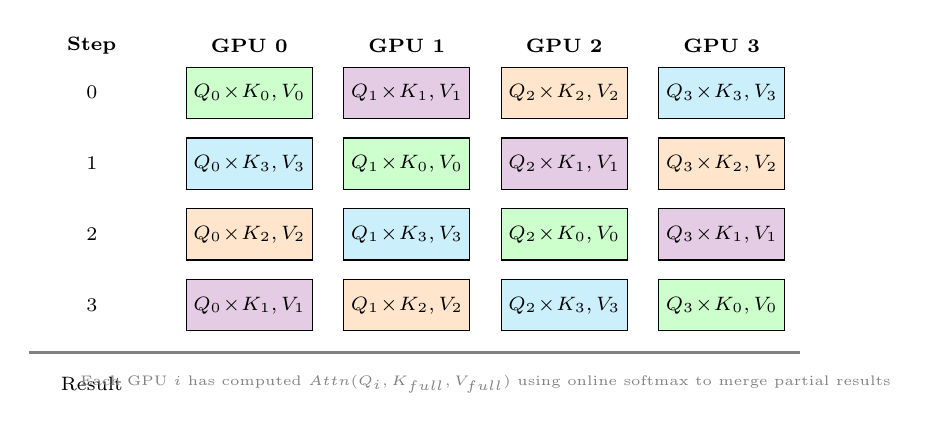
\begin{tikzpicture}[
    cell/.style={draw, minimum width=1.6cm, minimum height=0.65cm, font=\scriptsize, inner sep=2pt},
    hdr/.style={font=\scriptsize\bfseries},
    arr/.style={->, thick, >=stealth, blue!60},
    note/.style={font=\tiny, gray},
  ]
    % Headers
    \node[hdr] at (0, 0.6) {Step};
    \node[hdr] at (2.0, 0.6) {GPU 0};
    \node[hdr] at (4.0, 0.6) {GPU 1};
    \node[hdr] at (6.0, 0.6) {GPU 2};
    \node[hdr] at (8.0, 0.6) {GPU 3};

    % Step 0
    \node[font=\scriptsize] at (0, 0) {0};
    \node[cell, fill=green!20]  at (2.0, 0) {$Q_0 \!\times\! K_0,V_0$};
    \node[cell, fill=violet!20] at (4.0, 0) {$Q_1 \!\times\! K_1,V_1$};
    \node[cell, fill=orange!20] at (6.0, 0) {$Q_2 \!\times\! K_2,V_2$};
    \node[cell, fill=cyan!20]   at (8.0, 0) {$Q_3 \!\times\! K_3,V_3$};

    % Step 1
    \node[font=\scriptsize] at (0, -0.9) {1};
    \node[cell, fill=cyan!20]   at (2.0, -0.9) {$Q_0 \!\times\! K_3,V_3$};
    \node[cell, fill=green!20]  at (4.0, -0.9) {$Q_1 \!\times\! K_0,V_0$};
    \node[cell, fill=violet!20] at (6.0, -0.9) {$Q_2 \!\times\! K_1,V_1$};
    \node[cell, fill=orange!20] at (8.0, -0.9) {$Q_3 \!\times\! K_2,V_2$};

    % Step 2
    \node[font=\scriptsize] at (0, -1.8) {2};
    \node[cell, fill=orange!20] at (2.0, -1.8) {$Q_0 \!\times\! K_2,V_2$};
    \node[cell, fill=cyan!20]   at (4.0, -1.8) {$Q_1 \!\times\! K_3,V_3$};
    \node[cell, fill=green!20]  at (6.0, -1.8) {$Q_2 \!\times\! K_0,V_0$};
    \node[cell, fill=violet!20] at (8.0, -1.8) {$Q_3 \!\times\! K_1,V_1$};

    % Step 3
    \node[font=\scriptsize] at (0, -2.7) {3};
    \node[cell, fill=violet!20] at (2.0, -2.7) {$Q_0 \!\times\! K_1,V_1$};
    \node[cell, fill=orange!20] at (4.0, -2.7) {$Q_1 \!\times\! K_2,V_2$};
    \node[cell, fill=cyan!20]   at (6.0, -2.7) {$Q_2 \!\times\! K_3,V_3$};
    \node[cell, fill=green!20]  at (8.0, -2.7) {$Q_3 \!\times\! K_0,V_0$};

    % Result
    \draw[thick, gray] (-0.8, -3.3) -- (9.0, -3.3);
    \node[font=\scriptsize] at (0, -3.7) {Result};
    \node[note] at (5.0, -3.7) {Each GPU $i$ has computed $\text{Attn}(Q_i, K_\text{full}, V_\text{full})$ using online softmax to merge partial results};
  \end{tikzpicture}}
  \end{center}

  \vspace{0.3em}
  {\small
  \textbf{Communication--computation overlap:} While computing $\text{FlashAttn}(Q_i, K_j, V_j)$, the GPU simultaneously sends $K_j, V_j$ to its neighbor and receives $K_{j-1}, V_{j-1}$ from the other neighbor.
  }
\end{frame}

% -----------------------------------------------------------------------
\begin{frame}{Combining Partial Attention Results}

  Each ring step produces a partial attention output.  These are merged using the \textbf{online softmax} trick from Flash Attention.

  \vspace{0.3em}
  After processing block $j$, GPU $i$ maintains:
  \begin{description}[labelwidth=1.2cm]
    \item[$O_i$] Running weighted output accumulator
    \item[$\ell_i$] Running log-sum-exp (logsumexp of attention scores seen so far)
  \end{description}

  \vspace{0.2em}
  \begin{block}{Online merge of two partial results}
    Given partial outputs $(O_a, \ell_a)$ and $(O_b, \ell_b)$:
    \begin{align*}
      \ell_{\text{new}} &= \log\bigl(e^{\ell_a} + e^{\ell_b}\bigr) = \text{logaddexp}(\ell_a, \ell_b) \\
      O_{\text{new}} &= \frac{e^{\ell_a} \cdot O_a + e^{\ell_b} \cdot O_b}{e^{\ell_{\text{new}}}}
    \end{align*}
  \end{block}

  \vspace{0.2em}
  {\small
  \begin{itemize}
    \item This is \textbf{numerically stable} and produces the \textbf{exact same result} as computing attention over the full sequence
    \item The merge is $O(s/N_{\text{CP}} \cdot d)$ per step --- negligible compared to the attention computation
    \item Same principle used inside Flash Attention across SRAM tiles, here applied across GPUs
  \end{itemize}}
\end{frame}

% -----------------------------------------------------------------------
\begin{frame}{Causal Masking and Load Imbalance}

  \begin{columns}
    \begin{column}{0.48\textwidth}
      \textbf{Problem with na\"ive ring attention:}

      \vspace{0.2em}
      With causal masking, $Q_i$ can only attend to $K_j$ where $j \leq i$ (earlier tokens).

      \vspace{0.3em}
      \begin{center}
      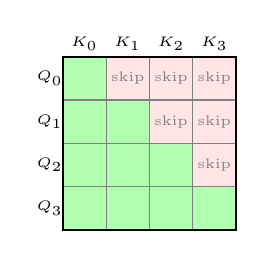
\begin{tikzpicture}[scale=0.55]
        % Lower triangle (computed)
        \fill[green!30] (0,3) rectangle ++(1,1);
        \fill[green!30] (0,2) rectangle ++(1,1); \fill[green!30] (1,2) rectangle ++(1,1);
        \fill[green!30] (0,1) rectangle ++(1,1); \fill[green!30] (1,1) rectangle ++(1,1); \fill[green!30] (2,1) rectangle ++(1,1);
        \fill[green!30] (0,0) rectangle ++(1,1); \fill[green!30] (1,0) rectangle ++(1,1); \fill[green!30] (2,0) rectangle ++(1,1); \fill[green!30] (3,0) rectangle ++(1,1);
        % Upper triangle (skipped)
        \fill[red!10] (1,3) rectangle ++(1,1); \fill[red!10] (2,3) rectangle ++(1,1); \fill[red!10] (3,3) rectangle ++(1,1);
        \fill[red!10] (2,2) rectangle ++(1,1); \fill[red!10] (3,2) rectangle ++(1,1);
        \fill[red!10] (3,1) rectangle ++(1,1);
        \node[font=\tiny, gray] at (1.5,3.5) {skip};
        \node[font=\tiny, gray] at (2.5,3.5) {skip};
        \node[font=\tiny, gray] at (3.5,3.5) {skip};
        \node[font=\tiny, gray] at (2.5,2.5) {skip};
        \node[font=\tiny, gray] at (3.5,2.5) {skip};
        \node[font=\tiny, gray] at (3.5,1.5) {skip};
        \draw[step=1, gray, thin] (0,0) grid (4,4);
        \draw[thick] (0,0) rectangle (4,4);
        % Labels
        \node[font=\tiny] at (0.5,4.3) {$K_0$};
        \node[font=\tiny] at (1.5,4.3) {$K_1$};
        \node[font=\tiny] at (2.5,4.3) {$K_2$};
        \node[font=\tiny] at (3.5,4.3) {$K_3$};
        \node[font=\tiny] at (-0.3,3.5) {$Q_0$};
        \node[font=\tiny] at (-0.3,2.5) {$Q_1$};
        \node[font=\tiny] at (-0.3,1.5) {$Q_2$};
        \node[font=\tiny] at (-0.3,0.5) {$Q_3$};
      \end{tikzpicture}
      \end{center}

      {\small GPU 0 computes 1 block, GPU 3 computes 4 blocks $\Rightarrow$ \textbf{load imbalance!}}
    \end{column}
    \begin{column}{0.48\textwidth}
      \textbf{Solution: Striped Attention}~\cite{brandon2023striped}

      \vspace{0.2em}
      Instead of contiguous chunks, assign tokens in a \emph{round-robin} (striped) pattern:

      \vspace{0.2em}
      {\small
      \begin{tabular}{ll}
        GPU 0: & tokens $0, 4, 8, 12, \ldots$ \\
        GPU 1: & tokens $1, 5, 9, 13, \ldots$ \\
        GPU 2: & tokens $2, 6, 10, 14, \ldots$ \\
        GPU 3: & tokens $3, 7, 11, 15, \ldots$
      \end{tabular}}

      \vspace{0.3em}
      \begin{center}
      \begin{tikzpicture}[scale=0.55]
        % All blocks computed (green background)
        \fill[green!30] (0,0) rectangle (4,4);
        % Diagonal blocks are half-full
        \fill[yellow!40] (0,3) rectangle ++(1,1);
        \fill[yellow!40] (1,2) rectangle ++(1,1);
        \fill[yellow!40] (2,1) rectangle ++(1,1);
        \fill[yellow!40] (3,0) rectangle ++(1,1);
        \node[font=\tiny] at (0.5,3.5) {$\sim\!\nicefrac{1}{2}$};
        \node[font=\tiny] at (1.5,2.5) {$\sim\!\nicefrac{1}{2}$};
        \node[font=\tiny] at (2.5,1.5) {$\sim\!\nicefrac{1}{2}$};
        \node[font=\tiny] at (3.5,0.5) {$\sim\!\nicefrac{1}{2}$};
        \draw[step=1, gray, thin] (0,0) grid (4,4);
        \draw[thick] (0,0) rectangle (4,4);
        % Labels
        \node[font=\tiny] at (0.5,4.3) {$K_0$};
        \node[font=\tiny] at (1.5,4.3) {$K_1$};
        \node[font=\tiny] at (2.5,4.3) {$K_2$};
        \node[font=\tiny] at (3.5,4.3) {$K_3$};
        \node[font=\tiny] at (-0.3,3.5) {$Q_0$};
        \node[font=\tiny] at (-0.3,2.5) {$Q_1$};
        \node[font=\tiny] at (-0.3,1.5) {$Q_2$};
        \node[font=\tiny] at (-0.3,0.5) {$Q_3$};
      \end{tikzpicture}
      \end{center}

      {\small Each GPU pair now has $\approx$ equal work $\Rightarrow$ balanced.}
    \end{column}
  \end{columns}
\end{frame}

% -----------------------------------------------------------------------
\begin{frame}{Context Parallelism --- Communication Analysis}

  Consider a single attention layer with $N_{\text{CP}}$ GPUs, sequence length $s$, hidden dim $d$, batch $b$.

  \vspace{0.3em}
  \textbf{Ring Attention:}
  \begin{itemize}
    \item Each step: send $K_j, V_j$ of shape $(b, s/N_\text{CP}, d)$ each $\Rightarrow$ $2 \cdot b \cdot \frac{s}{N_\text{CP}} \cdot d$ per step
    \item Total steps: $N_\text{CP} - 1$ (first block is local)
    \item Total volume per GPU: $2 \cdot b \cdot s \cdot d \cdot \frac{N_\text{CP} - 1}{N_\text{CP}}$
    \item \textbf{Overlapped} with $O\!\left(\frac{b \cdot s^2 \cdot d}{N_\text{CP}^2}\right)$ FLOPs of FlashAttn per step
  \end{itemize}

  \vspace{0.3em}
  \begin{alertblock}{When does overlap work?}
    Ring attention overlap is effective when computation per step $\gg$ communication per step, i.e.\ when $s / N_\text{CP}$ is large enough that FlashAttn time exceeds transfer time.
  \end{alertblock}
\end{frame}

% -----------------------------------------------------------------------
\begin{frame}{Context Parallelism --- Summary and Placement}

  \begin{columns}
    \begin{column}{0.48\textwidth}
      \textbf{Benefits}
      \begin{itemize}
        \item Enables training with very long sequences (100k--10M+ tokens)
        \item Linear memory reduction: activations per GPU $\propto s / N_{\text{CP}}$
        \item Orthogonal to TP, DP, PP --- can be combined freely
        \item Ring variant: communication overlaps with compute
      \end{itemize}

      \vspace{0.3em}
      \textbf{Limitations}
      \begin{itemize}
        \item Only helps when sequence length is the bottleneck (not model size)
        \item Ring: load imbalance with causal masking (needs striped attention)
        \item Additional implementation complexity
      \end{itemize}
    \end{column}
    \begin{column}{0.48\textwidth}
      \textbf{Typical 5D parallelism config:}

      \vspace{0.3em}
      {\small
      \begin{tabular}{l l}
        \toprule
        \textbf{Dimension} & \textbf{Scope} \\
        \midrule
        TP (+SP) & Intra-node (NVLink) \\
        CP       & Intra- or inter-node \\
        PP       & Inter-node \\
        DP/ZeRO  & Remaining GPUs \\
        \bottomrule
      \end{tabular}

      \vspace{0.3em}
      Total GPUs = $N_\text{TP} \times N_\text{CP} \times N_\text{PP} \times N_\text{DP}$
      }

      \vspace{0.5em}
      \textbf{When to use CP:}
      \begin{itemize}
        \item Sequence length $>$ 8k tokens
        \item Activation memory is the bottleneck
        \item After TP+SP is already applied within the node
      \end{itemize}
    \end{column}
  \end{columns}
\end{frame}

% -----------------------------------------------------------------------
\begin{frame}{Context Parallelism vs.\ Sequence Parallelism}

  \vspace{0.3em}
  \begin{center}
  {\small
  \begin{tabular}{l p{4.5cm} p{4.5cm}}
    \toprule
    & \textbf{Sequence Parallelism (SP)} & \textbf{Context Parallelism (CP)} \\
    \midrule
    \textbf{Scope} & Shards \emph{non-TP regions} (LayerNorm, Dropout) along $s$ & Shards \emph{attention and the full forward pass} along $s$ \\
    \textbf{Tied to TP?} & Yes --- always paired with TP & No --- orthogonal to TP \\
    \textbf{Communication} & AllGather / ReduceScatter within TP group & Point-to-point (ring) or AllToAll across CP group \\
    \textbf{Scales to} & Same node (TP limit) & Across nodes \\
    \textbf{Goal} & Reduce activation memory in non-TP ops & Enable very long sequences ($>$100k tokens) \\
    \bottomrule
  \end{tabular}}
  \end{center}

  \vspace{0.5em}
  \begin{alertblock}{Complementary, not competing}
    Use TP+SP inside a node and CP across nodes.  Both shard along the sequence dimension, but at different levels of the computation.
  \end{alertblock}
\end{frame}
